\documentclass[10pt]{article}
\usepackage[T1]{fontenc}
\usepackage[utf8]{inputenc}
\usepackage[brazil]{babel}
%\usepackage[math]{anttor} % fonte um pouco mais estilizada
\usepackage{import}
%\usepackage{parskip}
%=========================Packages==================================%
\usepackage{lscape,booktabs,latexsym,multicol,lmodern, natbib,graphicx,tikz,tkz-euclide,enumitem,fancyhdr, lipsum,siunitx, setspace,float}

\usepackage{amsmath,amsfonts,amssymb,amsthm}
\everymath{\displaystyle}

% configurações das questões, bem como: pontuação e estrutura.

\usepackage{tasks} % cria lista curta
\usepackage{exsheets} % cria questoes
\SetupExSheets[points]{name=ponto/s,number-format=\color{blue}} % define as configurações de pontuação das questões, e a cor da pontuação.

\DeclareInstance{exsheets-heading}{fancy-wp}{default}{
toc-reversed = true ,
indent-first = true ,
vscale = 2 ,
pre-code = \rule{\linewidth}{1pt} ,
post-code = \rule{\linewidth}{1pt} ,
title-format = \large\scshape\color{rgb:red,0.65;green,0.04;blue,0.07} ,
number-format = \large\bfseries\color{rgb:red,0.02;green,0.04;blue,0.48} ,
points-format = \itshape ,
points-pre-code = ( ,
points-post-code = ) ,
join =
{
number[r,B]title[l,B](.333em,0pt) ;
number[r,B]points[l,B](.333em,0pt)
} ,
attach = { main[hc,vc]number[hc,vc](0pt,0pt) }
}

%\SetupExSheets{headings=fancy-wp} % estilo diferente para o topo do enunciado com o nome " Exercício




\graphicspath{{imgs/}} %informa a pasta em que as imagens estão
%\usepackage{showframe} %Mostra linhas de marcação e margens
%FONTES
%\usepackage{fontspec}
%\usepackage{avant}
%\usepackage{mathptmx}
\usepackage{times}
%\usepackage[classicRfeIm]{kpfonts}
%\usepackage{kurier}


\usepackage{hyperref}% add hypertext capabilities
%\usepackage{txfonts}
%\usepackage{mathrsfs}

% CORES
\usepackage{xcolor}
\definecolor{corprimaria}{RGB}{10,48,123} 
\definecolor{corsecundaria}{RGB}{116,23,255}
\definecolor{corlinha}{RGB}{47,158,65}

\definecolor{corexercicio}{RGB}{38,38,38}
\definecolor{cordefinicao}{RGB}{47,158,65}
% \definecolor{corexemplo}{RGB}{116,23,255}
\definecolor{corexemplo}{RGB}{38,38,38}

% CORES DO PREPIF
\definecolor{cor1}{RGB}{239,239,239}
\definecolor{cor2}{RGB}{205,25,30}
\definecolor{cor3}{RGB}{47,158,65}
\definecolor{cor4}{RGB}{38,38,38}
\definecolor{cor5}{RGB}{28,28,28}

% ESTILOS
\newtheoremstyle{geral}% Nome do estilo do teorema
{0pt}% Espaço acima
{0pt}% Espaço abaixo
{\normalfont}% Fonte do corpo
{}% Indent amount
{\small\bf\sffamily\color{cor4}}% Theorem head font
{:}% Punctuation after theorem head
{0.25em}% Space after theorem head
{} % Optional theorem note

\newcounter{dummy}
\newcounter{Exer}
\newcounter{exer}
\newcounter{exem}
\theoremstyle{geral}
\newtheorem{ExercicioT}[Exer]{Exercício resolvido}
% \newtheorem{exercicioT}[exer]{ }
\newtheorem{definicaoT}[dummy]{Conceito}
\newtheorem{exemploT}[exem]{Exemplo}
\newtheorem{obsT}{Observação}

\RequirePackage[framemethod=default]{mdframed} % Required for creating the theorem, definition, exercise and corollary boxes

% Caixa de exercícios
\newmdenv[skipabove=7pt,
skipbelow=7pt,
rightline=false,
leftline=true,
topline=false,
bottomline=false,
backgroundcolor=corexercicio!10,
linecolor=corexercicio,
innerleftmargin=5pt,
innerrightmargin=5pt,
innertopmargin=5pt,
innerbottommargin=5pt,
leftmargin=0cm,
rightmargin=0cm,
linewidth=4pt]{caixaEx}	

% Caixa de definição
\newmdenv[skipabove=7pt,
skipbelow=7pt,
rightline=false,
leftline=true,
topline=false,
bottomline=false,
backgroundcolor=cordefinicao!10,
linecolor=cordefinicao,
innerleftmargin=5pt,
innerrightmargin=5pt,
innertopmargin=5pt,
innerbottommargin=5pt,
leftmargin=0cm,
rightmargin=0cm,
linewidth=4pt]{caixaDE}	

% Caixa de exemplos
\newmdenv[skipabove=7pt,
skipbelow=7pt,
rightline=false,
leftline=true,
topline=false,
bottomline=false,
backgroundcolor=corexemplo!10,
linecolor=corexemplo,
innerleftmargin=5pt,
innerrightmargin=5pt,
innertopmargin=5pt,
innerbottommargin=5pt,
leftmargin=0cm,
rightmargin=0cm,
linewidth=4pt]{caixaExem}	

% Caixa de observações	  
\newmdenv[skipabove=7pt,
skipbelow=7pt,
rightline=false,
leftline=true,
topline=false,
bottomline=false,
backgroundcolor=cor2!10,
linecolor=cor2,
innerleftmargin=5pt,
innerrightmargin=5pt,
innertopmargin=5pt,
innerbottommargin=5pt,
leftmargin=0cm,
rightmargin=0cm,
linewidth=4pt]{caixaObs}


\newenvironment{Exercicio}{\begin{caixaEx}\begin{ExercicioT}}{\end{ExercicioT}\end{caixaEx}}
% \newenvironment{exercicio}{\begin{caixaEx}\begin{exercicioT}}{\end{exercicioT}\end{caixaEx}}
\newenvironment{definicao}{\begin{caixaDE}\begin{definicaoT}}{\end{definicaoT}\end{caixaDE}}
\newenvironment{exemplo}{\begin{caixaExem} \begin{exemploT}}{\end{exemploT}\end{caixaExem}}

\newenvironment{obs}{\begin{caixaObs}\begin{obsT}}{\end{obsT}\end{caixaObs}}

\newenvironment{exercicio}[2][{\color{corexercicio}Exercício}]{\begin{trivlist}

\item[\hskip \labelsep {\bfseries #1}\hskip \labelsep {\bfseries #2.}]}{\end{trivlist}}


%===================================================
% MARGINS
%\usepackage[top=8mm, bottom=20mm, left=8mm, right=8mm]{geometry}
\usepackage{geometry}
\geometry{
	paper=a4paper, 
	top=2.5cm, 
	bottom=2.5cm, 
	left=1.5cm, 
	right=2cm,
	headheight=14pt, % Header height
	footskip=1.4cm, % Espaço da margem inferior à linha de base do rodapé
	headsep=10pt, % Espaço da margem superior até a linha de base do cabeçalho
	%showframe, % Uncomment to show how the type block is set on the page
}


% NOVOS COMANDOS
\newcommand{\atv}{Lista de Exercícios 00}
\newcommand{\preceptor}{Monitor: Matheus Jonatha}




% CABEÇALHO E RODAPÉ
\pagestyle{fancy}
%\lfoot{\notaesquerda}
\cfoot{}
\rfoot{{\color{white}\thepage}}
%\lhead{HELLO}
%\chead{HELLO}
%\rhead{\textbf{The performance of new graduates}}
\renewcommand{\headrulewidth}{0pt} %linha horizontal no topo da pagina
%\renewcommand{\footrulewidth}{0.4pt} %linha horizontal no pé da pagina

%\setlength\parindent{0pt}
%\setlength\parskip{1.5ex}
%\setlength\parsep{1.5\parskip}
%\thispagestyle{empty}%\bigskip %Rodapé na primeira pagina


%para nao ficar o retangulo em volta dos links, apenas muda a cor dos caracteres
\hypersetup{ colorlinks,
linkcolor=blue,
filecolor=blue,
urlcolor=blue,
citecolor=blue }



% QUESTÕES
% configurações das questões, bem como: pontuação e estrutura.

\usepackage{tasks} % cria lista curta
\usepackage{exsheets} % cria questoes
\SetupExSheets[points]{ name=ponto/s,number-format=\color{blue}} % define as configurações de pontuação das questões, e a cor da pontuação.

\DeclareInstance{exsheets-heading}{fancy-wp}{default}{
toc-reversed = true ,
indent-first = true ,
vscale = 2 ,
pre-code = \rule{\linewidth}{1pt} ,
post-code = \rule{\linewidth}{1pt} ,
title-format = \large\scshape\color{rgb:red,0.65;green,0.04;blue,0.07} ,
number-format = \large\bfseries\color{rgb:red,0.02;green,0.04;blue,0.48} ,
points-format = \itshape ,
points-pre-code = ( ,
points-post-code = ) ,
join =
{
number[r,B]title[l,B](.333em,0pt) ;
number[r,B]points[l,B](.333em,0pt)
} ,
attach = { main[hc,vc]number[hc,vc](0pt,0pt) }
}

%\SetupExSheets{headings=fancy-wp} % estilo diferente para o topo do enunciado com o nome " Exercício
\usepackage{capt-of}%%To get the caption

\hypersetup{pdfauthor={Matheus Jonatha},
            pdftitle={Conjutos Numéricos},
            pdfsubject={PrepIF - Material de Matemática},
            pdfkeywords={conjuntos,numéricos,numericos,mathjonatha,mthsjonatha,matematica,prepif,if,preparatorio,online,instituto,federal,militares,material},
            pdfproducer={Produzido e gerado no Overleaf},
            pdfcreator={pdflatex}}
\begin{document}
    \import{estrutura/}{background.tex} % CAPA
        \begin{center}
            {\LARGE {\sc conjuntos numéricos}}
        \end{center}

\begin{definicao}
Conjunto é o agrupamento de elementos que possuem as mesmas características. Quando esses elementos são números, essa união passa a ser conhecida como \textbf{conjunto numérico}. Na matemática, pode-se agrupar os números de diversas formas, gerando assim muitos conjuntos numéricos.
\end{definicao}

\section*{Conjunto dos números naturais (\( \mathbb{N} \))}
É o conjunto representado pela letra \( \mathbb{N}\) e dele podemos citar algumas características importantes:

    \begin{enumerate}[label=\textbf{(\Roman*)}]
        \item Representamos sua forma como sendo \( \mathbb{N} = \{0, 1, 2, 3, 4, \ldots, n, \ldots\}\).
        \item É um conjunto infinito. Os pontinhos (\(\ldots\)) informam que continua infinitamente.
        \item Sabemos exatamente quais são os sucessores \((n+1)\) e os antecessores \((n-1)\) de cada um dos seus elementos.
        
        \begin{obs}
        Essa informação de como escrever o sucessor e o antecessor de um número é importante para questões que necessitam de generalização nos cálculos, Bem como saber a representação genérica de um número par (\(2n\)) e de um número ímpar (\(2n+1\)).
        \end{obs}
        \item O número zero é o único que não tem antecessor.
        \item Ao realizar às operações de edição ou multiplicação entre dois de seus elementos, obtemos como resultado um elemento desse mesmo conjunto.
    \end{enumerate}
\subsection*{Subconjuntos de \( \mathbb{N} \)}
Subconjunto é a parte de um conjunto com características próprias. Veja alguns exemplos abaixo:

\begin{multicols}{2}
    \begin{itemize}
        \item Conjunto dos números naturais não nulos:
        
            \( \mathbb{N}^* = \{1, 2, 3, 4, \ldots \} \)
        \item Conjunto dos números naturais pares:
            
            \( \mathbb{N}_p = \{2, 4, 6, 8, \ldots \} \)
        \item Conjunto dos números naturais ímpares:
        
            \( \mathbb{N}_i = \{1, 3, 5, 7, \ldots \} \)
        \item Conjunto dos números naturais primos:
        
            \( C = \{2, 3, 5, 7, 11, 13, \ldots \} \)
        
    \end{itemize}
\columnbreak
\bigskip
\noindent
    \begin{minipage}{\linewidth}
        \centering 
        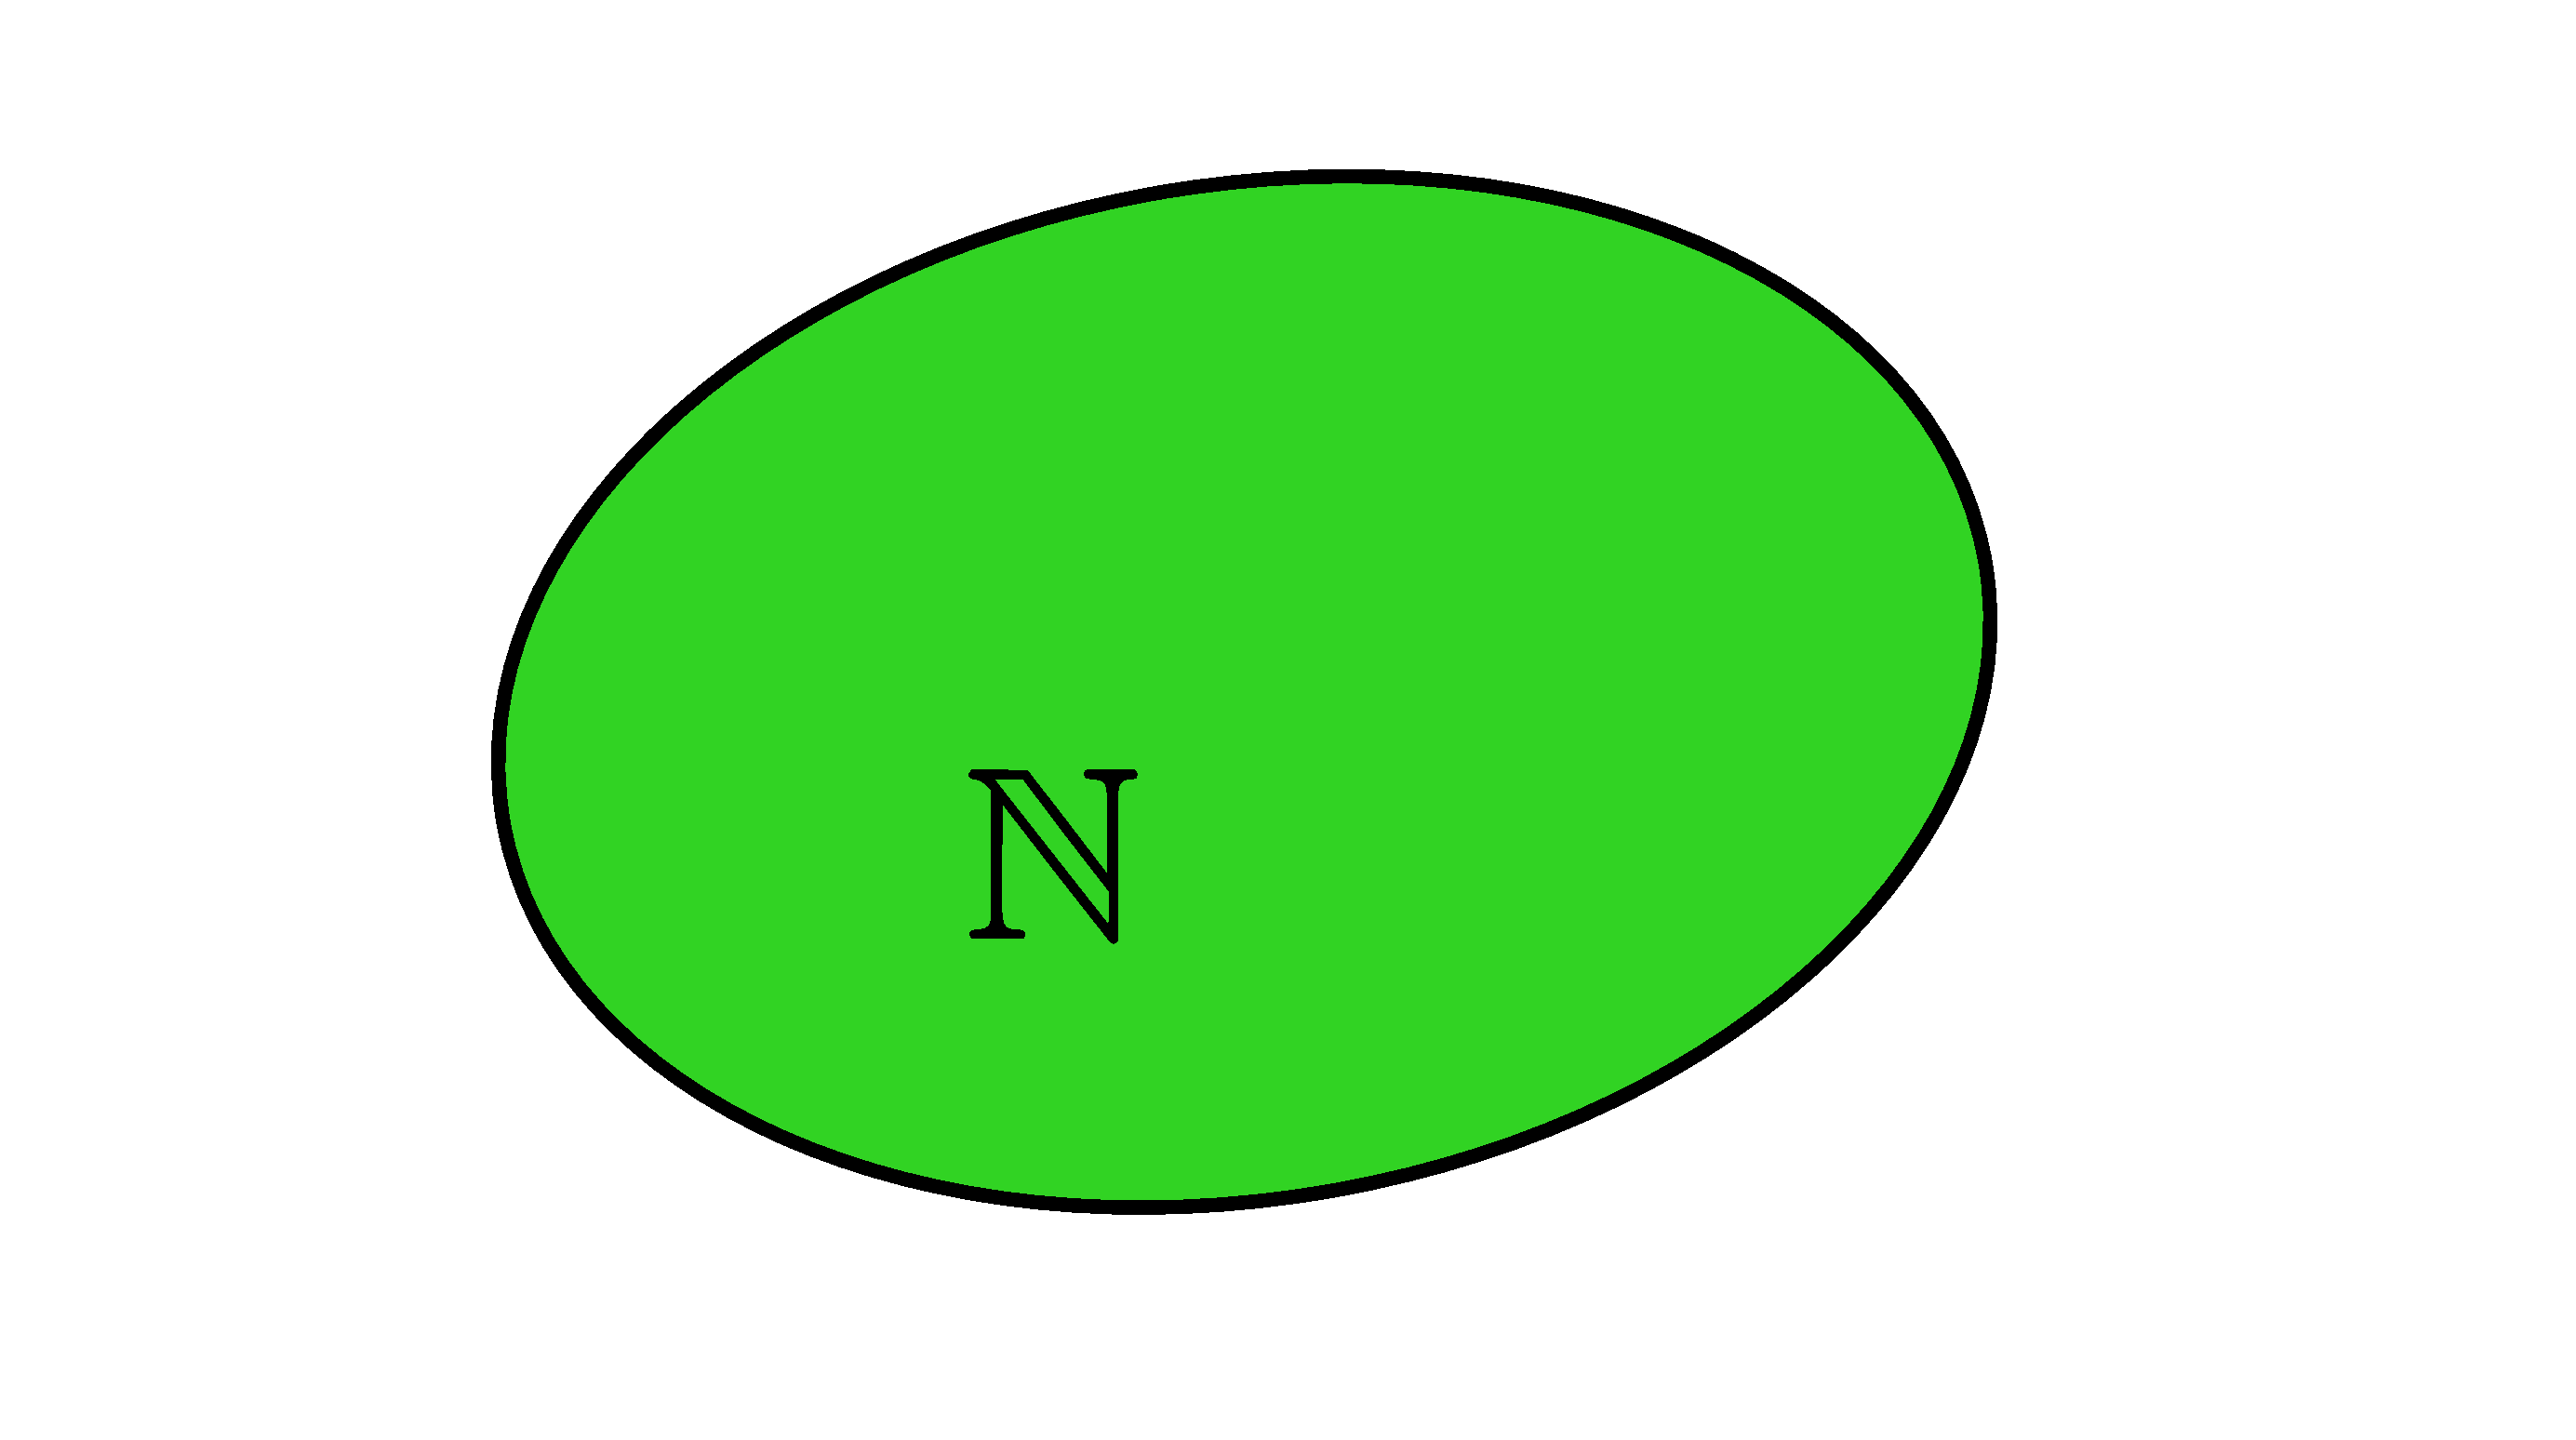
\includegraphics[width=0.8\textwidth]{imgs/conjuntosNumerico/conjuntosNaturais.pdf}
        \captionof{figure}{Representação do conjunto dos números naturais.}
        \label{fig:conjuntosNaturais} 
    \end{minipage}%
\end{multicols} 



\section*{Conjunto dos números inteiros (\( \mathbb{Z} \))}
O conjunto dos números naturais é um subconjunto dos inteiros (Figura \ref{fig:conjuntosInteiros}), representados pelo \( \mathbb{Z}\). As suas características são:

    \begin{enumerate}[label=\textbf{(\Roman*)}]
        \item O conjunto é formado pelos números naturais e seus simétricos negativos (opostos), incluindo o zero.
            \begin{obs}
                Há uma diferença entre \textbf{oposto de um número} e \textbf{inverso de um número}. Um número é oposto de outro quando a soma desses dois números resultar em zero, já o inverso será uma fração com numerador 1 e o denominador o número que será invertido.
                \textbf{Exemplos:}
                \begin{enumerate}
                    \begin{multicols}{2}
                        \item O oposto do número \(34\) é \( -34 \)
                        \item O oposto do número \(62\) é \( -62 \)
                        \item O inverso do número \(28\) é \( \frac{1}{28} \)
                        \item O inverso do número \(246\) é \( \frac{1}{246} \)
                    \end{multicols}
                \end{enumerate}
            \end{obs}
\newpage
\import{estrutura/}{background.tex} % CAPA
        \item Sua forma é representada como \( \mathbb{Z} = \{\ldots, -3, -2, -1, 0, 1, 2, 3, \ldots\}\).
        \item É um conjunto infinito.
        \item Sabemos exatamente quais são os sucessores e os antecessores de cada um dos seus elementos.
        \item O número zero possui sucessor e antecessor.
        \item Ao realizar as operações de adição, subtração e multiplicação entre dois de seus elementos, obtemos como resultado um elemento desse mesmo conjunto.
    \end{enumerate}
\subsection*{Subconjuntos de \( \mathbb{Z} \)}

\begin{multicols}{2}
    \begin{itemize}
        \item Conjunto dos números inteiros não nulos:

            \( \mathbb{Z}^* = \{\ldots, -3, -2, -1, 1, 2, 3, \ldots \} \)
        \item Conjunto dos números inteiros não negativos:
            
            \( \mathbb{Z}_+ = \{0, 1, 2, 3, \ldots \} \)
            
            \begin{obs}
            Note que esse subconjunto é o mesmo que o conjunto dos números naturais, logo, podemos dizer que \( \mathbb{N} = \mathbb{Z}_+\)
            \end{obs}
        \item Conjunto dos números inteiros positivos:
        
            \( \mathbb{Z}^*_+ = \{1, 2, 3, \ldots \} \)
        \item Conjunto dos números inteiros não positivos:
        
            \( \mathbb{Z}_- = \{\ldots, -4, -3, -2, -1, 0 \} \)
        \item Conjunto dos números inteiros negativos:
        
            \( \mathbb{Z}^*_- = \{\ldots, -5, -4, -3, -2, -1\} \)
        
    \end{itemize}
\columnbreak
\bigskip
\noindent
    \begin{minipage}{\linewidth}
        \centering 
        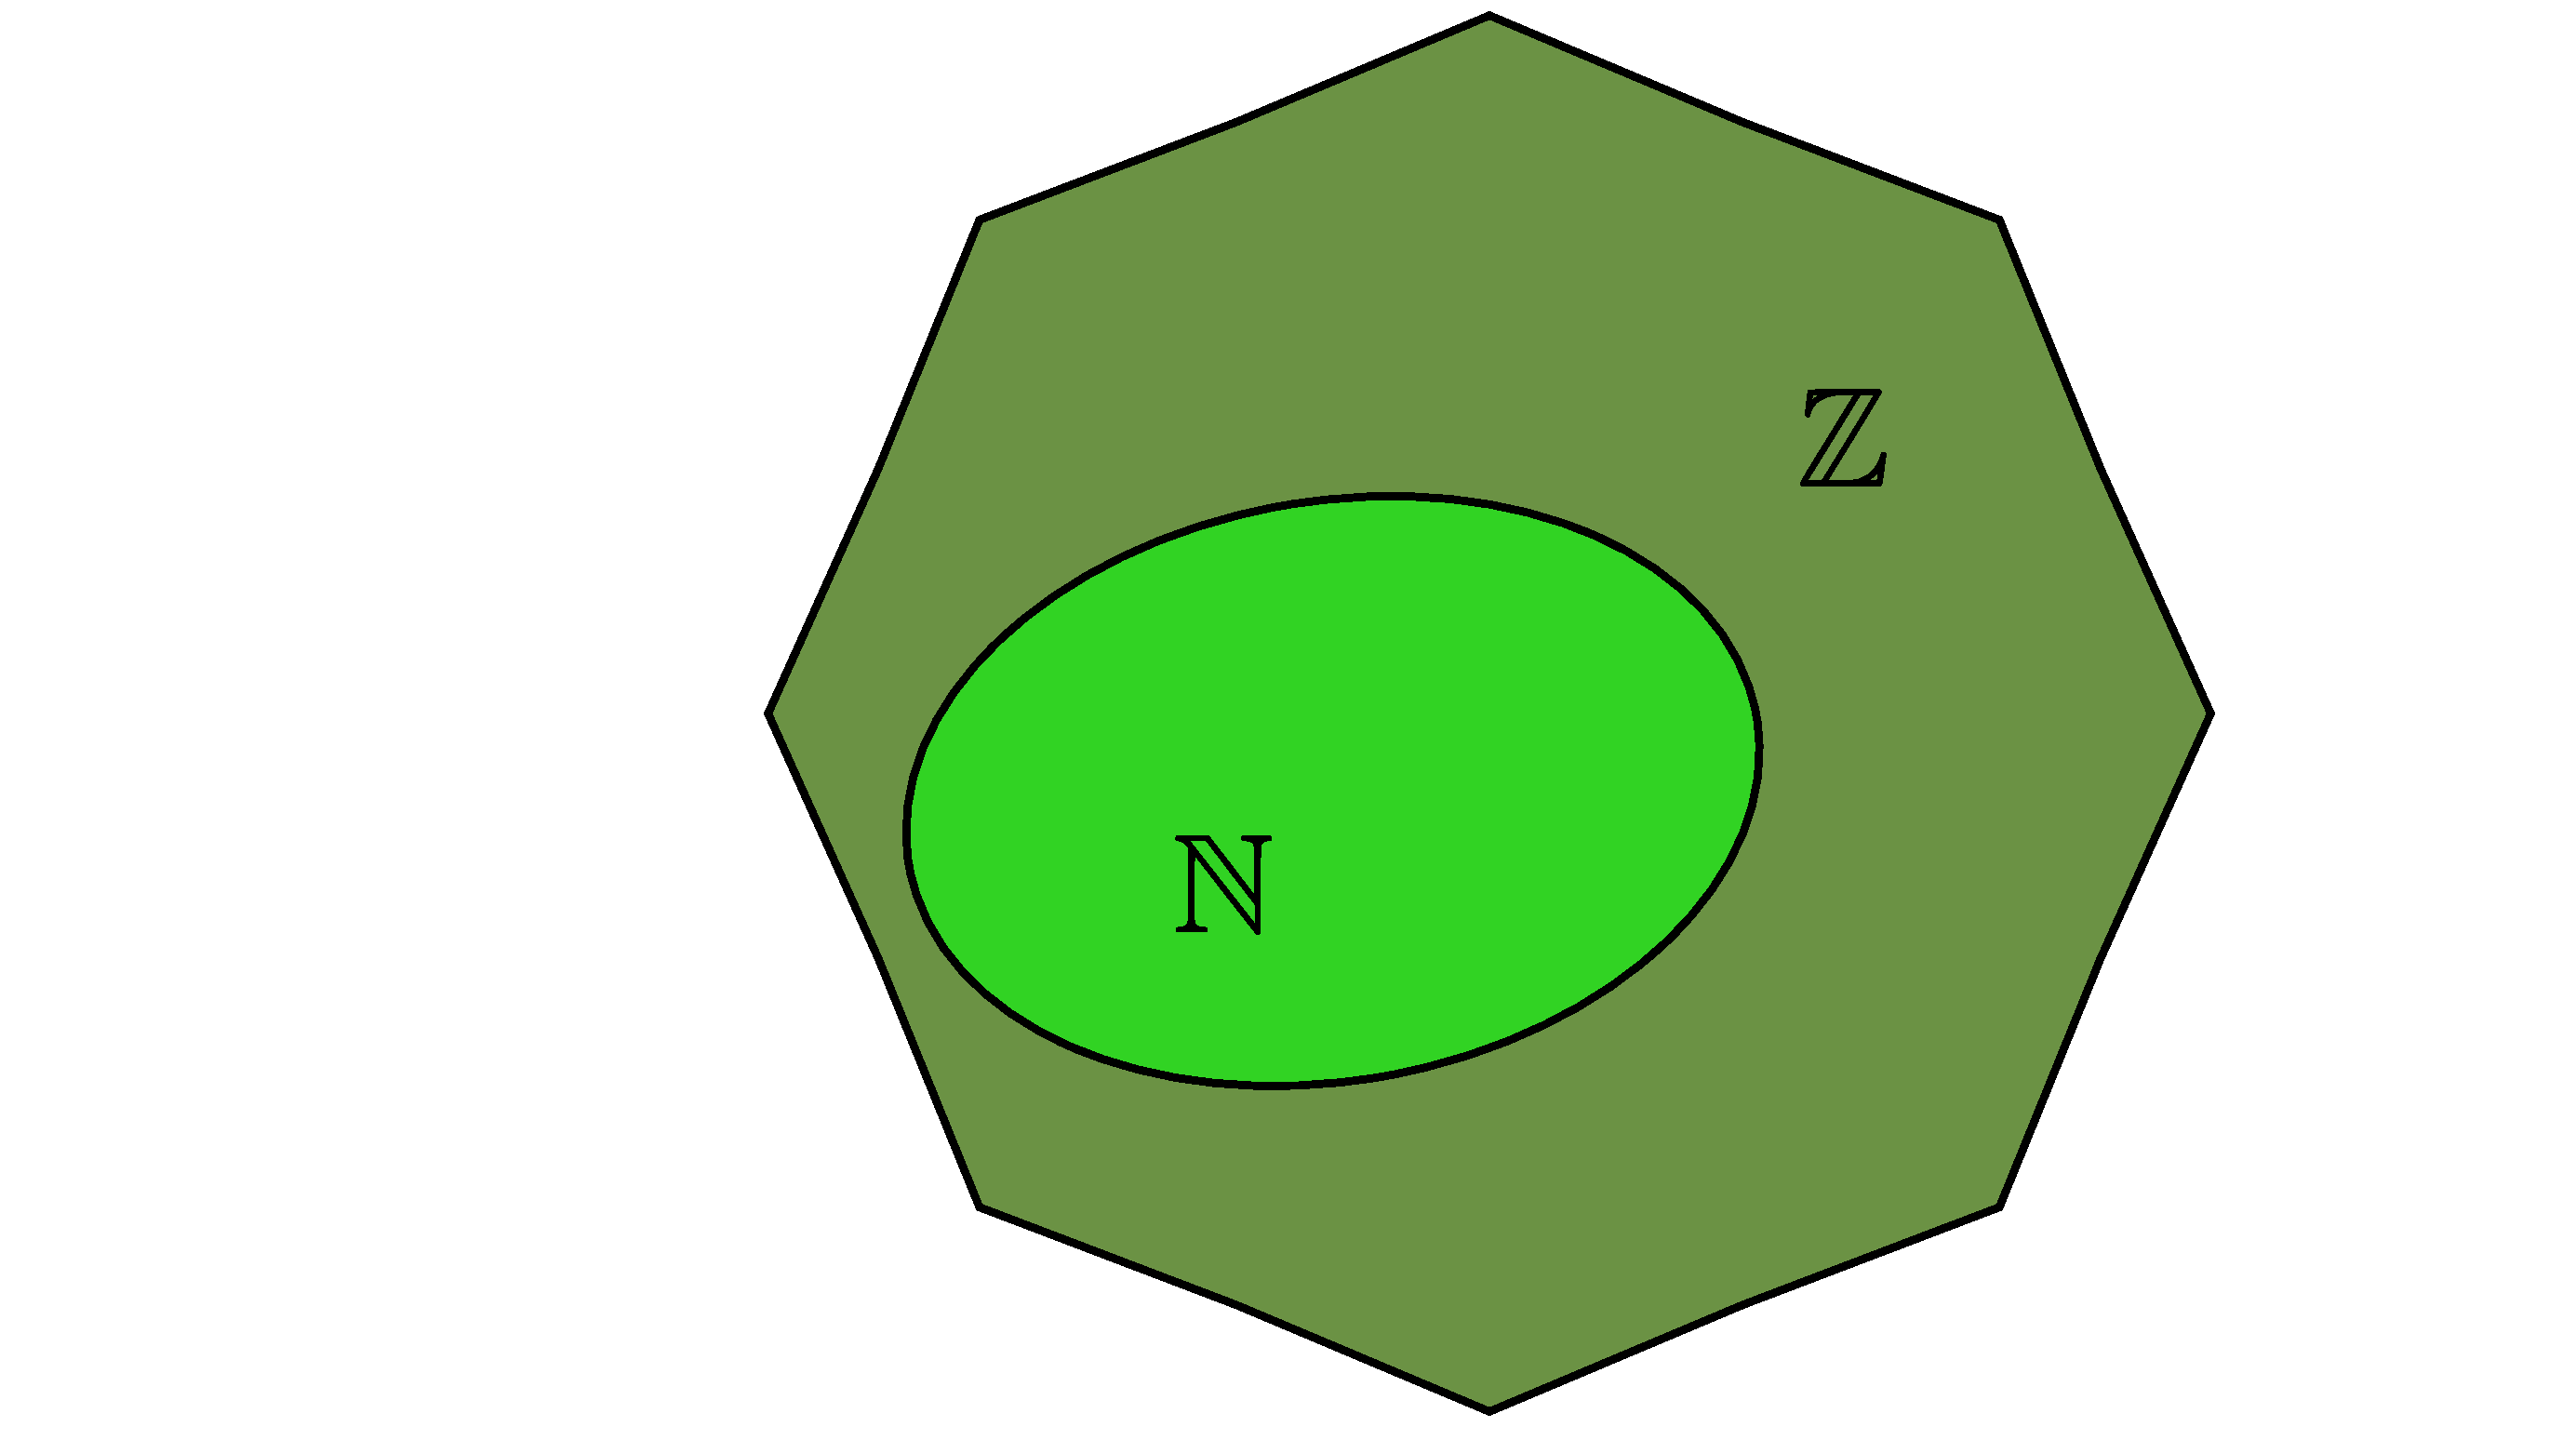
\includegraphics[width=0.8\textwidth]{imgs/conjuntosNumerico/conjuntosInteiros.pdf}
        \captionof{figure}{Representação do conjunto dos números inteiros.}
        \label{fig:conjuntosInteiros} 
    \end{minipage}%
\end{multicols} 

\section*{Conjunto dos números racionais (\( \mathbb{Q} \))}
O conjunto dos números racionais pode ser escrito como o quociente (fração) entre dois números inteiros, \( a \) e \(  b \in \mathbb{Z} \) e \( b \neq 0 \), em outras palavras, definimos como:
\[ \mathbb{Q} = \left\{ \frac{a}{b} \mid  a \textrm{ e } b \in \textrm{ e } b \neq 0 \right\} \]

\begin{enumerate}[label=\textbf{(\Roman*)}]
        \item O conjunto dos números inteiros (\(\mathbb{Z}\)) está contido nesse conjunto, ou seja, é um subconjunto do conjunto dos números racionais.
        \begin{obs}
        Podemos escrever a situação acima como \( \mathbb{Z} \subset \mathbb{Q} \) ou \( \mathbb{Q} \supset \mathbb{Z} \). O símbolo \( \subset \) lê-se \textbf{está contido} e \( \supset \) lê-se \textbf{contém}.
        \end{obs}
        \item Entre dois números inteiros ou racionais, existem infinitos números racionais.
        \item Podemos escrever qualquer número inteiro na forma racional, basta adicionar o número 1 ao denominador.
        
        \textbf{Exemplo:} O número inteiro \( 28 \) pode ser escrito como sendo \( \frac{28}{1} \).
        \item  Ao realizar as operações de adição, subtração e multiplicação entre dois números racionais, obtemos como resultado um número inteiro ou racional.
\end{enumerate}
\newpage
\import{estrutura/}{background.tex} % CAPA
\subsection*{Subconjuntos de \( \mathbb{Q} \)}
\begin{multicols}{2}
    \begin{itemize}
        \item \( \mathbb{Q}^* \): Conjunto dos números racionais não nulos:
        \item \( \mathbb{Q}_+ \): Conjunto dos números racionais não negativos:
        \item \( \mathbb{Q}^*_+ \): Conjunto dos números racionais positivos:
        \item  \( \mathbb{Q}_- \): Conjunto dos números racionais não positivos:
        \item  \( \mathbb{Q}^*_- \): Conjunto dos números racionais negativas:
    \end{itemize}
\columnbreak
\bigskip
\noindent
    \begin{minipage}{\linewidth}
        \centering 
        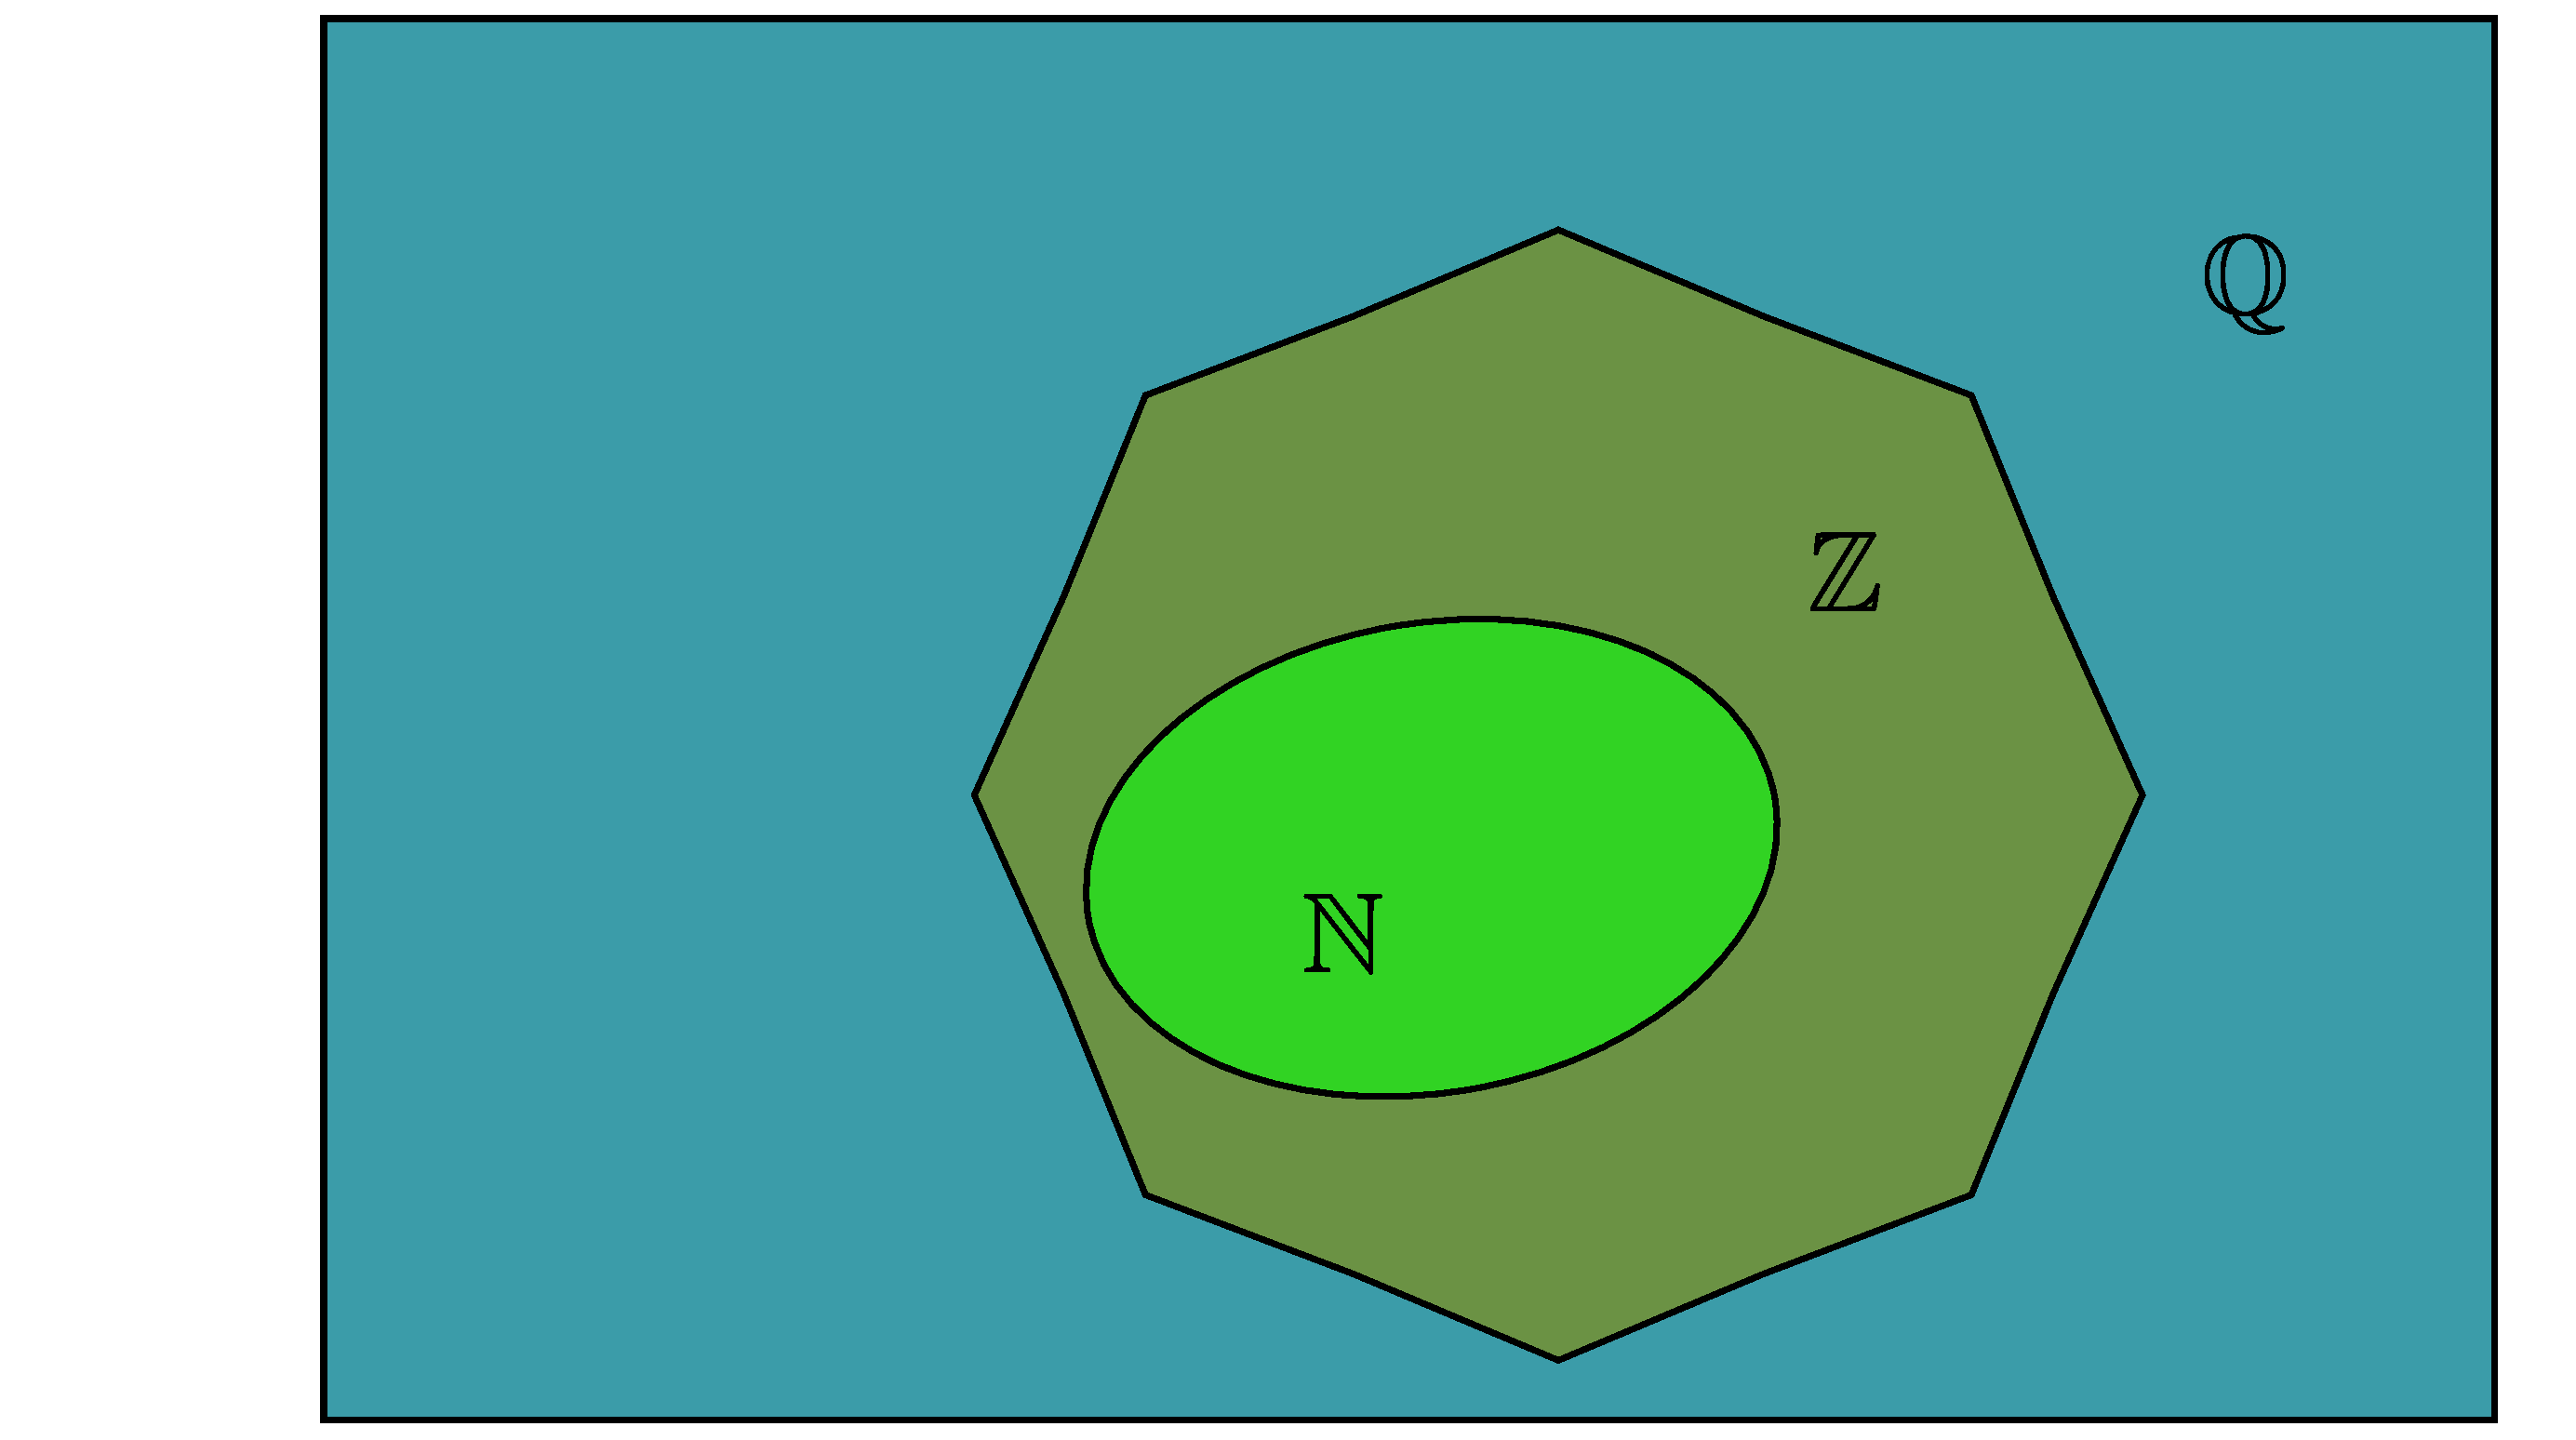
\includegraphics[width=0.8\textwidth]{imgs/conjuntosNumerico/conjuntosRacionais.pdf}
        \captionof{figure}{Representação do conjunto dos números racionais.}
        \label{fig:conjuntosRacionais} 
    \end{minipage}%
\end{multicols} 


\section*{Conjunto dos números irracionais (\( \mathbb{I} \))}
O conjunto dos números irracionais é aquele cujos elementos são números decimais que não podem ser resultado da divisão entre dois números inteiros. Essa definição é o oposto da definição de número racional: qualquer número que pode ser escrito na forma de fração.
    \begin{enumerate}[label=\textbf{(\Roman*)}]
            \item É formado pelos números decimais infinitos e não periódicos.
\begin{multicols}{2}
            \item Exemplos de números irracionais são: 
                    \begin{itemize}
                        \item \( \pi = 3,141592\ldots\)
                        \item \( \sqrt{2} = 1,4142135\ldots\)
                        \item \( \sqrt{3}= 1,7320508\ldots\)
                        \item \( \sqrt{1+ \sqrt{3}}\)
                        \item \( 24, 51465163\ldots \)
                        \item \( \sqrt[3]{5} \)
                    \end{itemize}
\columnbreak
\bigskip
\noindent
    \begin{minipage}{\linewidth}
        \centering 
        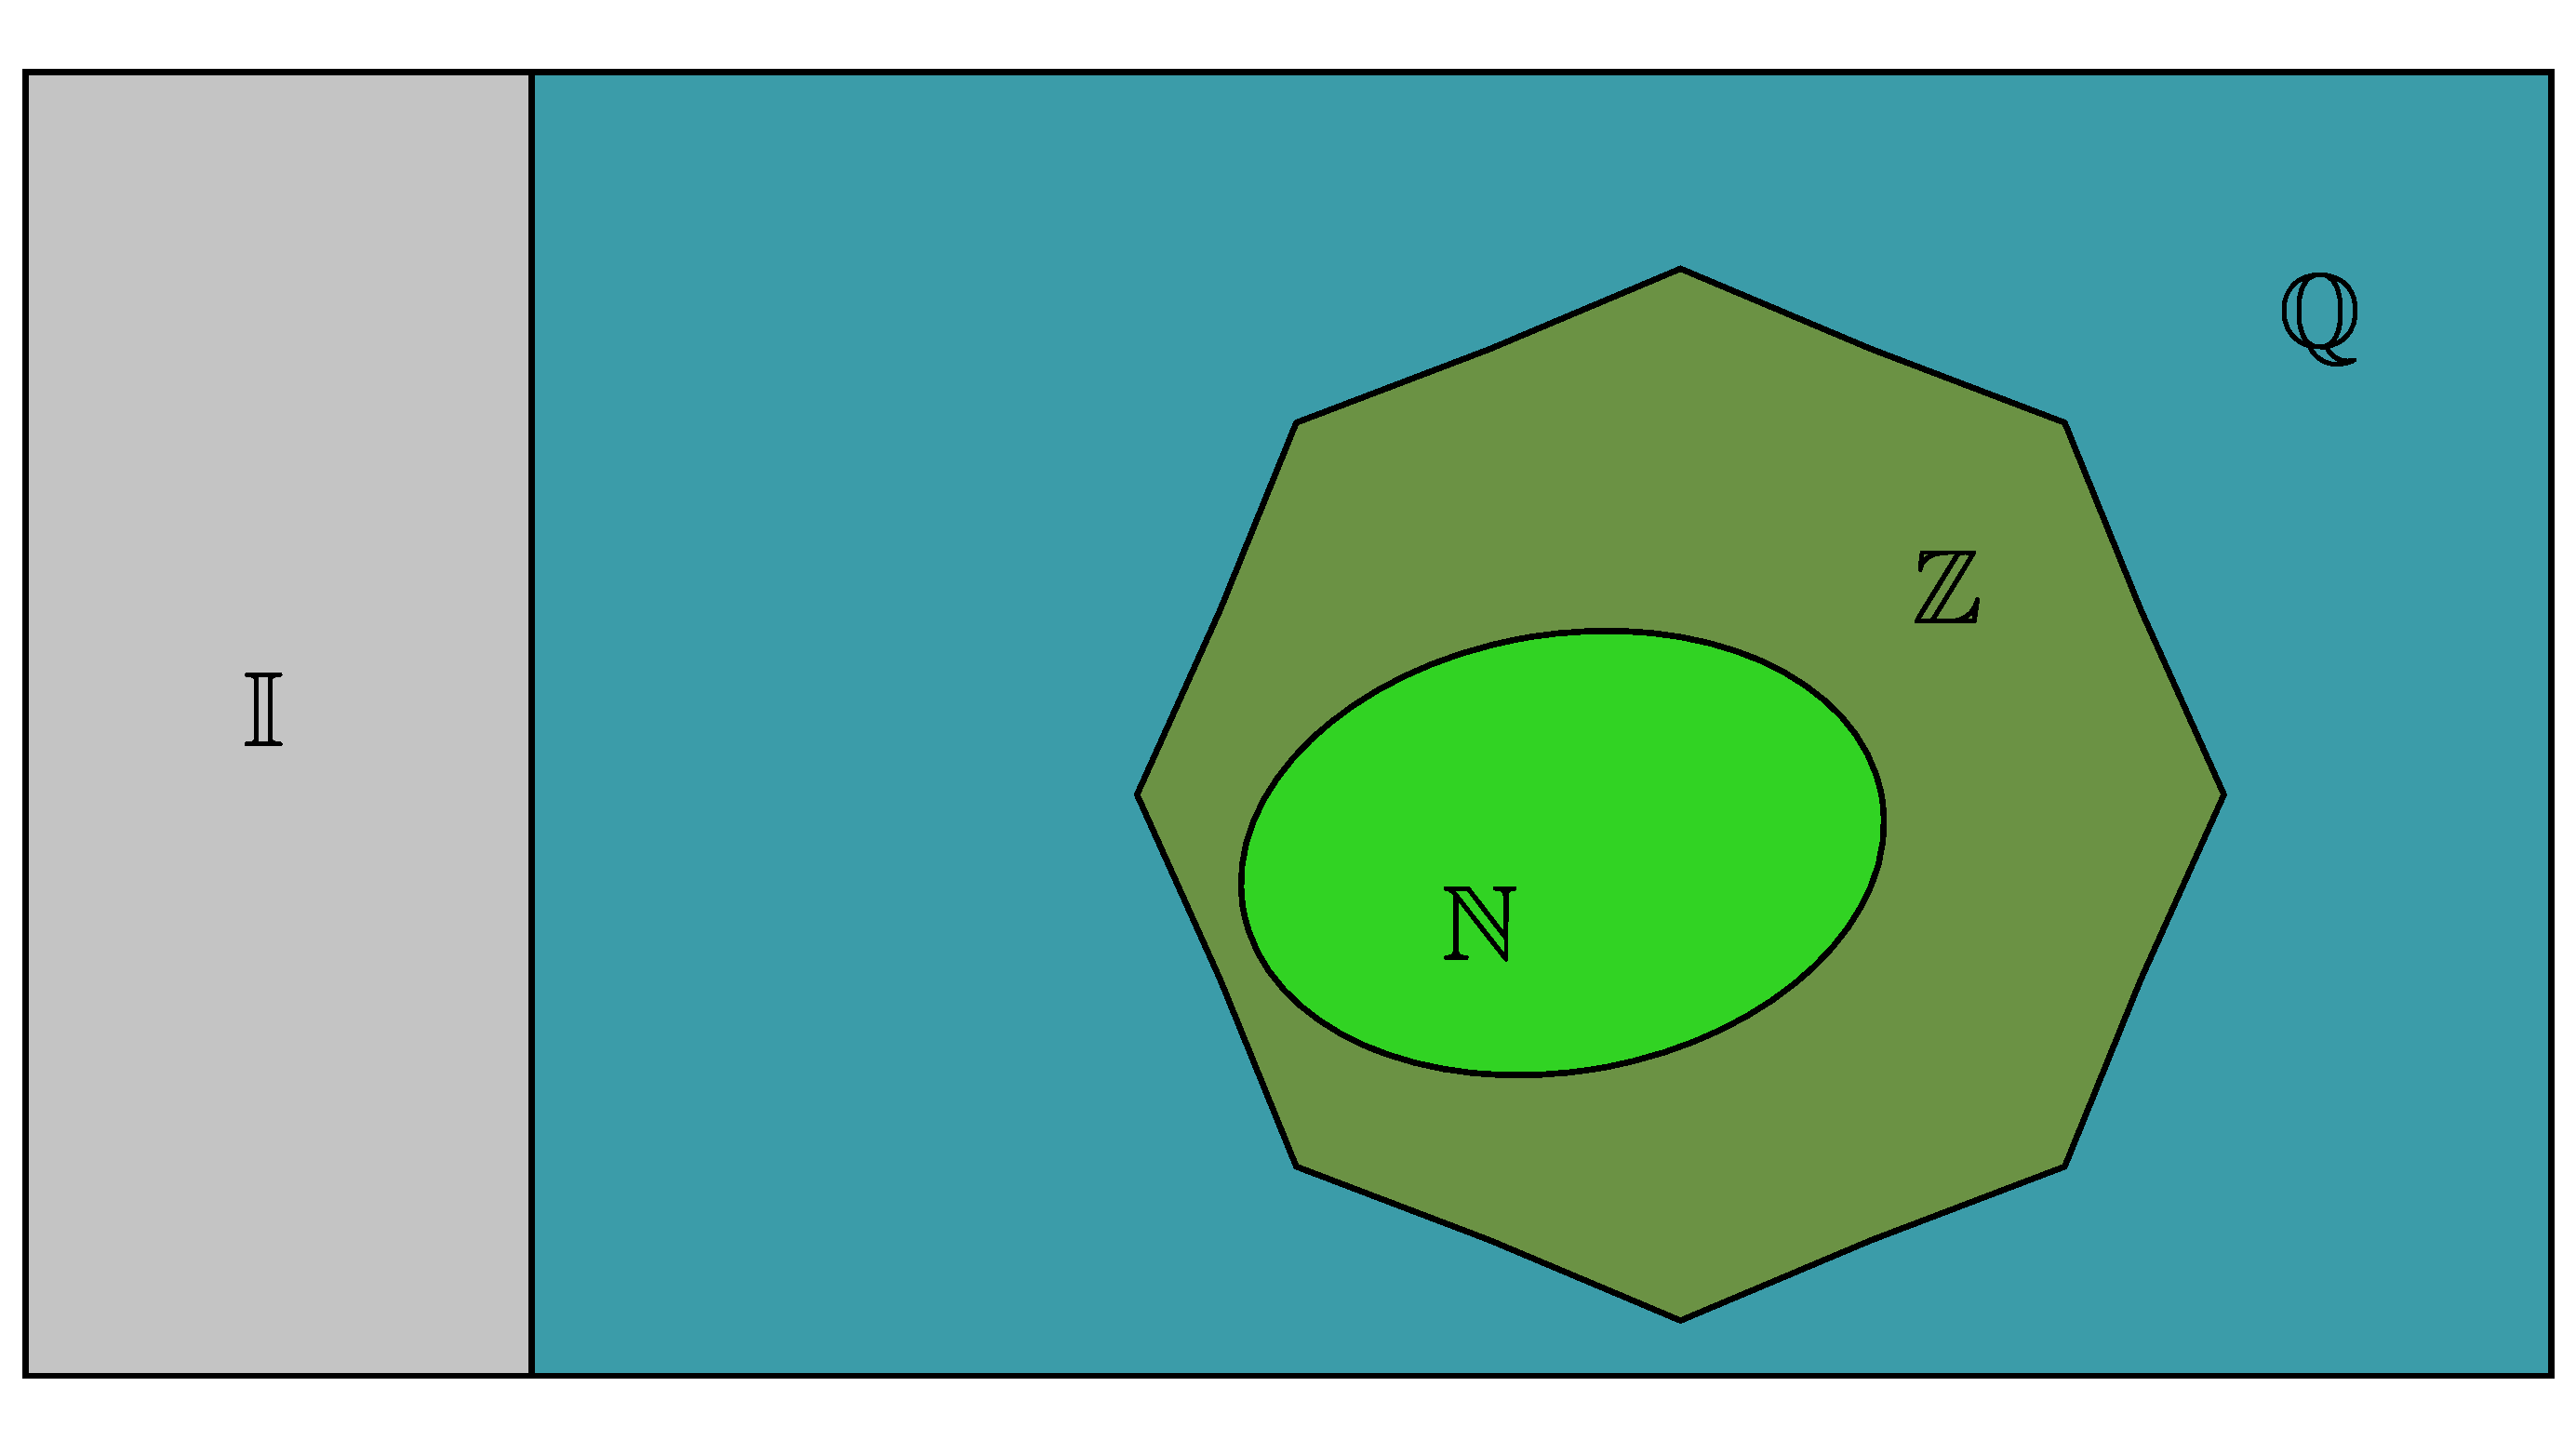
\includegraphics[width=0.8\textwidth]{imgs/conjuntosNumerico/conjuntosIrracionais.pdf}
        \captionof{figure}{Representação do conjunto dos números irracionais.}
        \label{fig:conjuntosIrracionais} 
    \end{minipage}%
\end{multicols} 
            \item A soma, subtração, multiplicação ou divisão de dois irracionais pode resultar em um racional ou em um irracional.
    \end{enumerate}
\section*{Conjunto dos números reais (\( \mathbb{R} \))}
O conjunto dos números reais (\( \mathbb{R} \)) é formado pela reunião(união) do conjunto dos números racionais (\( \mathbb{Q}\)) com o conjunto dos números irracionais (\( \mathbb{I}\)), ou seja, por todos os conjuntos que estudamos até o momento. A relação entre todos os conjuntos pode ser representada como mostrado na figura \ref{fig:conjuntosReais}:
\begin{multicols}{2}
\subsection*{Subconjuntos de \(\mathbb{R}\)}
\begin{itemize}
        \item \( \mathbb{R}^* \): Conjunto dos números reais não nulos:
        \item \( \mathbb{R}_+ \): Conjunto dos números reais não negativos:
        \item \( \mathbb{R}^*_+ \): Conjunto dos números reais positivos:
        \item  \( \mathbb{R}_- \): Conjunto dos números reais não positivos:
        \item  \( \mathbb{R}^*_- \): Conjunto dos números reais negativas:
    \end{itemize}
\columnbreak
\bigskip
\noindent
    \begin{minipage}{\linewidth}
        \centering 
        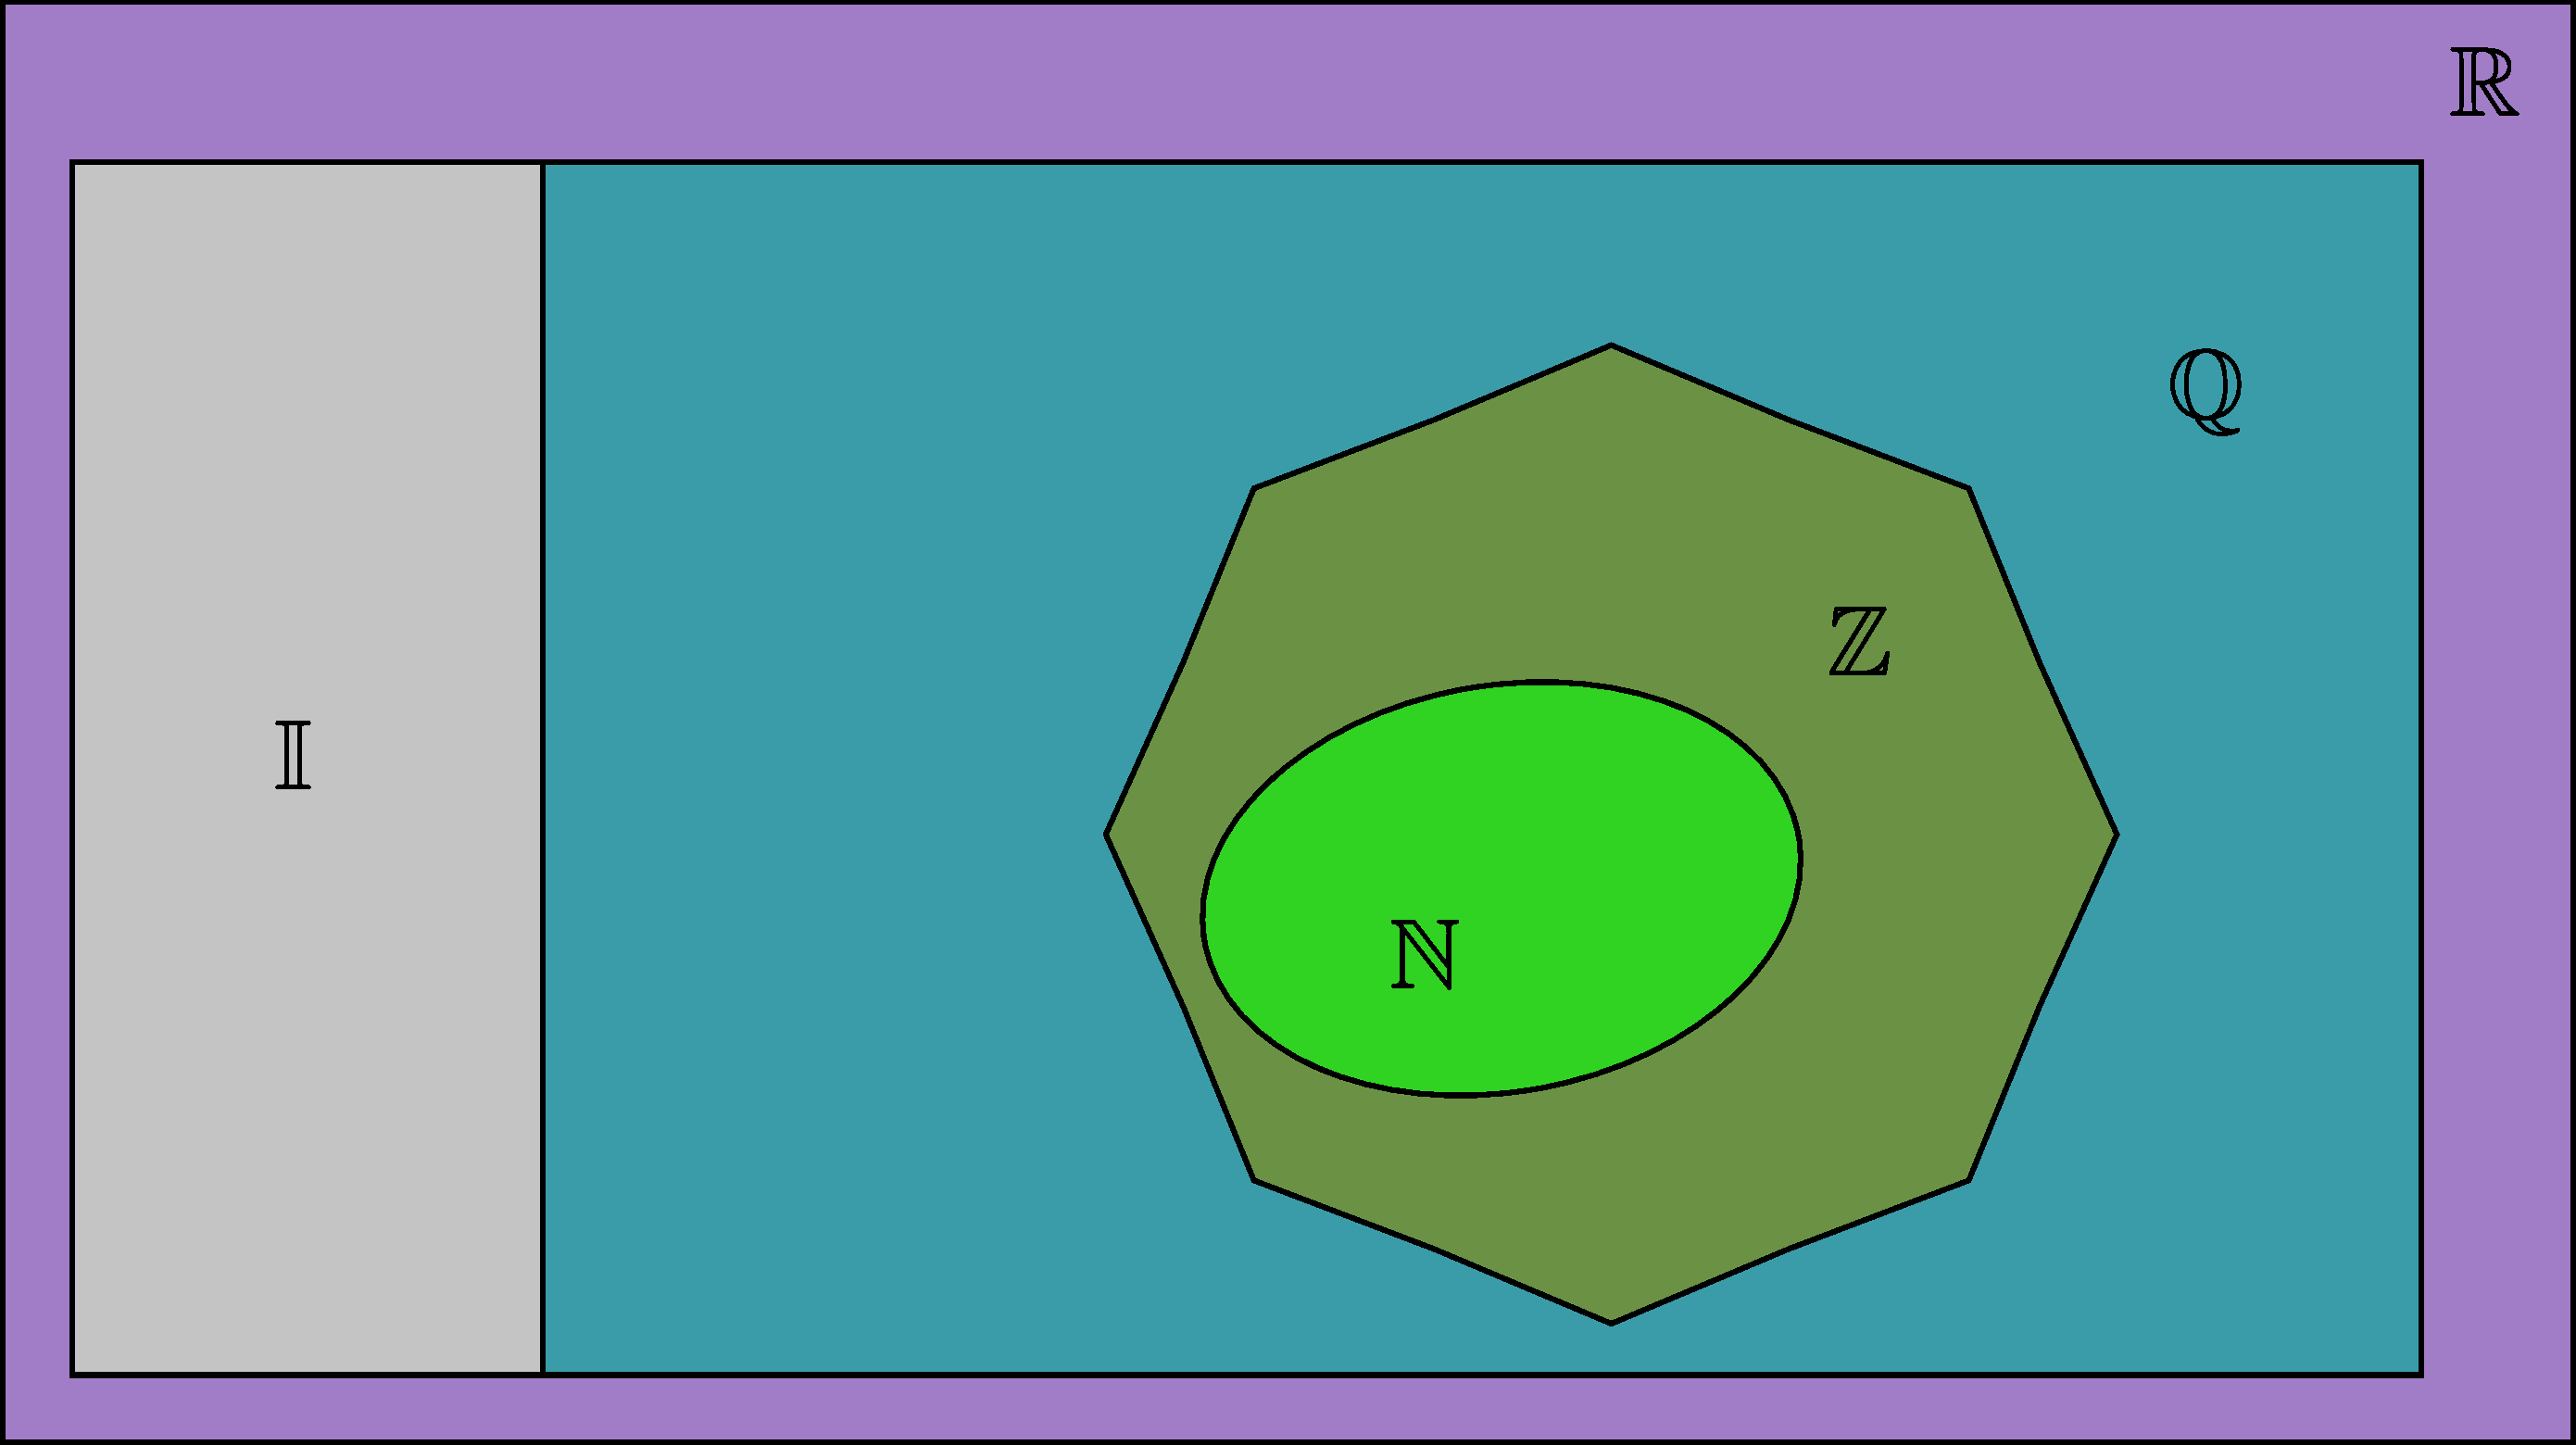
\includegraphics[width=0.8\textwidth]{imgs/conjuntosNumerico/conjuntosReais.pdf}
        \captionof{figure}{Representação do conjunto dos números reais.}
        \label{fig:conjuntosReais} 
    \end{minipage}%
\end{multicols} 
\newpage
\import{estrutura/}{background.tex} % CAPA

 \begin{center}
            {\LARGE {\sc hora de praticar}}
        \end{center}

Nesta seção, você encontra exercícios de fixação. Tente realizar todos, pois o conteúdo mostrado anteriormente é utilizado como ferramenta no desenvolvimento das questões. É importante lembrar que uma questão dificilmente vai te pedir uma informação sobre conjuntos numéricos de forma direta,esse conteúdo é utilizado como \textbf{ferramenta} para encontrar o resultado final (não é o único caminho, mas é um atalho).

As resoluções das questões podem ser encontradas no nosso \href{https://prepif.herokuapp.com/instituicoes}{site}. No enunciado das questões, são informados o instituto, o ano e o número da questão (ex.: \textbf{IFRN2020Q12}).

\begin{multicols}{2}
\setlength\columnseprule{1pt}
\def\columnseprulecolor{\color{corlinha}}%

\begin{question}[name = Questão]
\textbf{IFCE2018Q37}
A solução real positiva da equação 

\noindent\( x^2 - \sqrt{2} \cdot x - 12 = 0 \) é o número

\begin{tasks}(1)
        \task \( 2\sqrt{2} \)
        \task \( 3\sqrt{2} \)
        \task \( \sqrt{2} \)
        \task \( 4\sqrt{2} \)
        \task \( 5\sqrt{2} \)
    \end{tasks}
\end{question}

\begin{question}[name = Questão]
\textbf{IFCE2018Q39}
O quadrilátero \( ABCD \) é tal que os ângulos \( A\widehat{B}C\) e \( A\widehat{D}C\) são retos. Sabendo que os lados \( AB \), \( BC \) e \( CD \) medem \( 7\mathrm{m} \), \( 24\mathrm{m} \) e \( 20\mathrm{m} \), respectivamente, podemos concluir que o perímetro desse quadrilátero, em \(\mathrm{m} \), vale

\begin{tasks}
        \task \( 66 \)
        \task \( 62 \)
        \task \( 51 \)
        \task \( 54 \)
        \task \( 70 \)
    \end{tasks}
\end{question}

\begin{question}[name = Questão]
\textbf{IFCE2017Q38}
Um triângulo retângulo que tem um cateto medindo \( 5 \) e cuja hipotenusa mede \( 13 \) tem área igual a

\begin{tasks}(1)
        \task \( 30 \)
        \task \( 65 \)
        \task \( 18 \)
        \task \( 60 \)
        \task \( 32,5 \)
    \end{tasks}
\end{question}

\begin{question}[name = Questão]
\textbf{IFCE2017Q40}
Um triângulo possui dois lados medindo \( 4 \mathrm{cm}\) que formam um ângulo de \( 120^\circ \). O outro lado desse triângulo e a altura relativa a esse lado têm medidas, em centímetros, respectivamente iguais a

\begin{tasks}(1)
        \task \( 2\sqrt{3} \) e \( 2 \)  
        \task \( 4 \) e \( 4\sqrt{3} \)  
        \task \( 4\sqrt{3} \) e \( 2 \)  
        \task \( 2\sqrt{3} \) e \( \sqrt{3} \)  
        \task \( 2 \) e \( \sqrt{3} \)  
    \end{tasks}
\end{question}

\end{multicols}

\vfill
\section*{Referências}
\noindent Disponível em: \url{https://beduka.com/blog/materias/matematica/resumo-de-conjuntos-numericos/}. Acesso em: 8 de agosto de 2020.

\noindent Disponível em: 
\url{https://bit.ly/2Cp7I3X}. Acesso em: 9 de agosto de 2020.

\noindent Disponível em: 
\url{https://www.stoodi.com.br/resumos/matematica/conjuntos-numericos/}. Acesso em: 10 de agosto de 2020.

\end{document}